\chapter{Существующие алгоритмы} \label{ch:ch2}

\section{Анализ} \label{sec:ch2/sec1}

В основном в качестве источника информации используются статьи \cite{dai, hodge, vakili, varun, billor, wilkinson}. Помимо статей интерес представляют датасеты, которые тоже предстояло найти. Среди датасетов есть хорошо известный MNIST с набором изображений рукописных цифр, а также данные о разных сортах винных изделий, свободных электронах в ионосфере Земли, о заболеваниях сердца и другие.

В этой работе рассматриваются стационарные данные. Поиск аномалий во временных рядах, а также прогнозирование временных рядов находятся за рамками рассматриваемой в работе темы.

\section{Основы алгоритмов} \label{sec:ch2/sec2}

Задачу поиска аномалий можно отнести к классу задач обучения без учителя. Суть поиска аномалий заключается в том, чтобы найти в выборке объекты, которые не похожи на большинство объектов выборки, т. е. те, которые выделяются на фоне других.

Часто бывает так, что аномальных объектов либо нет вообще, либо их очень мало и неизвестно где именно в выборке они находятся. Поэтому поиск аномалий относится к классу задач обучения без учителя (т. к. отсутствуют размеченные данные).

\section{Результат работы алгоритмов} \label{sec:ch1/sec2}

Результатом работы алгоритма для поиска аномалий могут быть как \textbf{степени аномалии} (anomaly scores), так и \textbf{бинарные метки} (binary labels).

В случае, когда алгоритм выдаёт \textbf{степень аномалии}, под степенью понимается уровень вероятности того, что объект является выбросом (аномалией).

В случае \textbf{бинарных меток} алгоритм сразу указывает на нормальные (обычно обозначаемые как 0) и аномальные (обозначаемые как 1) данные. Несмотря на то, что некоторые алгоритмы детектирования аномалий возвращают бинарные метки напрямую, степени аномалий тоже могут быть переведены в бинарное представление. 0 или 1 содержат меньше информации, чем степень аномалии. Тем не менее, это конечный результат, по которому обычно принимается решение об аномальности объекта выборки.

\section{Классификация методов определения аномалий} \label{sec:ch1/sec3}

Большинство методов определения аномалий используют метки, по которым можно определить, является ли объект выборки нормальным или аномальным. Поиск или сбор размеченных данных, которые будут точными и хорошо описывать рассматриваемую проблемы, чтобы хорошо обучить алгоритмы, довольно сложно и дорого.

\noindent Обычно выделяют три типа методов поиска аномалий:

\begin{enumerate}
	\item \textbf{Supervised методы (обучение с учителем)}

Предполагается, что имеется доступ к обучающим данным с точными и репрезентативными метками для нормальных и аномальных объектов. В таком случае обычно разрабатывают предсказательную модель для обоих классов. После обучения на тренировочных данных к каждому объекту из тестовой выборки применяется алгоритм, чтобы определить класс объекта. 
%\todo{Однако есть и проблема: получить точные и репрезентативные метки, особенно для аномалий, сложно. Поскольку аномалия определяется через смесь нескольких атрибутов. Такая ситуация довольно распространена в сценариях, таких как обнаружение мошенников в потоке информации в банковском секторе (сложно отличить мошенника от обычного пользователя только по действиям).}
	
	\item \textbf{Semi-supervised методы (обучение с частичным привлечение учителя)}

Предполагается, что имеются размеченные данные только для нормального класса. Так как для обучения таких алгоритмов не требуются размеченные аномальные данные, они имеют более широкое применение, чем supervised методы.
	\item \textbf{Unsupervised методы (обучение без учителя)}

Такие методы не требуют обучающих данных и поэтому наиболее широко используются. Unsupervised методы поиска аномалий могут нормальные данные из всех представленных и рассматривать отклонение от них как аномалию.
\end{enumerate}
Многие semi-supervised методы могут быть использованы для unsupervised случая. Например, с их помощью можно дополнительно семплировать объекты из выборки, если данных для обучения алгоритма попросту недостаточно.

\subsection{Метрика качества модели}

В качестве основной метрики используется ROC-AUC, что расшифровывается как receiver operating characteristic -- area under curve и переводится как "рабочая характеристика приёмника -- площадь под кривой". ROC-кривая позволяет оценить качество бинарной классификации\footnote{бинарная означает, что есть лишь два класса объектов -- например, нормальные и аномальные}. Она показывает соотношение между долей объектов, которые были верно классифицированы как принадлежащие определённому классу (True Positive Rate, TPR), от общего числа объектов в выборке Именно площадь под кривой и выступает в роли метрики качества. Минимальное значение, которое может принимать ROC-AUC составляет 0.5, а максимальное -- 1. 

%Дальше будет описано чем это вызвано.

%\todo{ROC-кривая (англ. receiver operating characteristic, рабочая характеристика приёмника) — график, позволяющий оценить качество бинарной классификации, отображает соотношение между долей объектов от общего количества носителей признака, верно классифицированных как несущих признак, (англ. true positive rate, TPR, называемой чувствительностью алгоритма классификации) и долей объектов от общего количества объектов, не несущих признака, ошибочно классифицированных как несущих признак (англ. false positive rate, FPR, величина 1-FPR называется специфичностью алгоритма классификации) при варьировании порога решающего правила. Также известна как кривая ошибок. Анализ классификаций с применением ROC-кривых называется ROC-анализом. Количественную интерпретацию ROC даёт показатель AUC (англ. area under ROC curve, площадь под ROC-кривой) — площадь, ограниченная ROC-кривой и осью доли ложных положительных классификаций. Чем выше показатель AUC, тем качественнее классификатор, при этом значение 0,5 демонстрирует непригодность выбранного метода классификации (соответствует случайному гаданию). Значение менее 0,5 говорит, что классификатор действует с точностью до наоборот: если положительные назвать отрицательными и наоборот, классификатор будет работать лучше.}

\begin{figure}[ht]
  \centering
  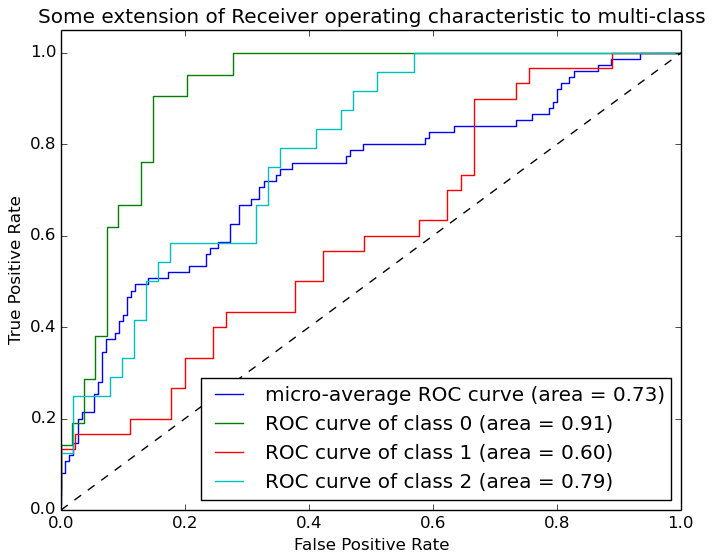
\includegraphics [scale=0.7] {roc_curve}
  \caption{Пример ROC-кривой.}
  \label{fig:roc_curve}
\end{figure}

График на рисунке \ref{fig:roc_curve} был построен с помощью библиотеки scikit-learn\footnote{\url{https://scikit-learn.org/0.15/auto_examples/plot_roc.html}}.

\clearpage

\section{Подходы к решению} \label{sec:ch2/sec3}

Одним из возможных способов определения аномалий является измерение схожести между объектов. У такого способа есть два варианта:
\begin{enumerate}
  \item Восстановление плотности
  \item Классификация
\end{enumerate}

\subsection{Восстановление плотности}

В случае с восстановлением плотности необходимо построить распределение, которое хорошо описывает выборку. И это распределение позволяет посчитать вероятность для нового объекта получить его из распределения, описывающего выборку.

В терминах этого метода аномалия - объект, полученный из другого распределения, описывающего другую выборку данных.

\noindent Есть три подхода:
\begin{enumerate}
  \item Параметрический
  \item Непараметрический
  \item Восстановление смесей
\end{enumerate}

\noindent\textbf{Параметрический метод} -- Распределение представляется в виде $p(x)=\phi(x\vert\theta)$, где $\theta$ выступает в качестве параметра распределения. Например, в семейство параметрических распределений входит распределение Гаусса - $\theta=(\mu, \Sigma)$, где $\mu$ - вектор средних и $\Sigma$ - ковариационная матрица.

Параметры модели подбираются таким образом, чтобы вероятность объектов из обучающей выборки была максимальной. Для этого обычно пользуются Методом Максимального Правдоподобия:

\[ \sum_{i}\log\phi(x_{i}\vert\theta) \rightarrow \max_{\theta} \]

%Есть ещё Автокодировщики, которые хорошо справляются с понижением размерности данных и с помощью которых можно хорошо семплировать из заданного распределения \cite{karazeev}.

\clearpage

\section{Алгоритмы} \label{sec:ch2/sec4}

\noindent В текущей работе были рассмотрены следующие алгоритмы:

\begin{enumerate}
	\item k-Nearest Neighbors (k-NN) \cite{knn} -- метод k-ближайших соседей.
	\item Principal Component Analysis (PCA) \cite{pca} -- метод главных компонент.
	\item One-Class Support Vector Machines (OCSVM) \cite{ocsvm} -- одноклассовый метод опорных векторов.
	\item Local Outlier Factor (LOF) \cite{lof} -- метод локального уровеня выброса.
	\item Histogram-Based Outlier Score (HBOS) \cite{hbos} -- оценка выбросов на основе гистограммы.
	\item Isolation Forest \cite{iforest} -- метод изолируещего леса.
\end{enumerate}

%\subsection{k-Nearest Neighbors (k-NN)}
%
%
%
%\subsection{Principal Component Analysis (PCA)}
%
%
%
%\subsection{One-Class Support Vector Machines (OCSVM)}
%
%
%
%\subsection{Local Outlier Factor (LOF)}
%
%
%
%\subsection{Histogram-Based Outlier Score (HBOS)}
%
%
%
%\subsection{Isolation Forest}



\clearpage



\section{Датасеты} \label{sec:ch2/sec5}



\noindent Для проверки сервиса были рассмотрены следующие датасеты:
\begin{enumerate}
  \item Arrhythmia -- определение наличия аритмии по данным ЭКГ \cite{guvenir}.
  \item Breast Cancer -- определение типа опухоли молочной железы: доброкачественная или злокачественная.
  \item Glass -- идентификация типа стекла, оставленного на месте преступления.
  \item Ionosphere -- рассматриваются характеристики радаров, которые используется в анализе ионосферы: необходимо определить является радар "плохим" или "хорошим".
  \item Letter Recognition -- по описанию изображения определить присутствует ли буква из английского алфавита или нет.
  \item Mammography -- детектирование микрокальцинатов по данным маммографии.
  \item MNIST -- научиться различать изображения рукописных цифр 6 и 0.
  \item Satellite -- определение типа почвы по спутниковым снимкам.
\end{enumerate}
В качестве источника этих данных выступает библиотека ODDS \cite{odds}.

\begin{table} [htbp]
	\centering
	\caption{Статистика по данным из рассматриваемых датасетов.}\label{tab:stats}%
	\begin{tabular}{lrrr}
		\toprule
		     Датасет & Кол-во объектов & Размерность &  Процент выбросов \\
		\midrule
		  arrhythmia &      452 &         274 &      14.60 \\
		     breastw &      683 &           9 &      34.99 \\
		       glass &      214 &           9 &       4.21 \\
		  ionosphere &      351 &          33 &      35.90 \\
		      letter &     1600 &          32 &       6.25 \\
		 mammography &    11183 &           6 &       2.33 \\
		       mnist &     7603 &         100 &       9.21 \\
		   satellite &     6435 &          36 &      31.64 \\
		\bottomrule
		\hline
	\end{tabular}
\end{table}

Сравнение данных, которые представлены в указанных датасетах.

\begin{figure}[ht]
  \centering
  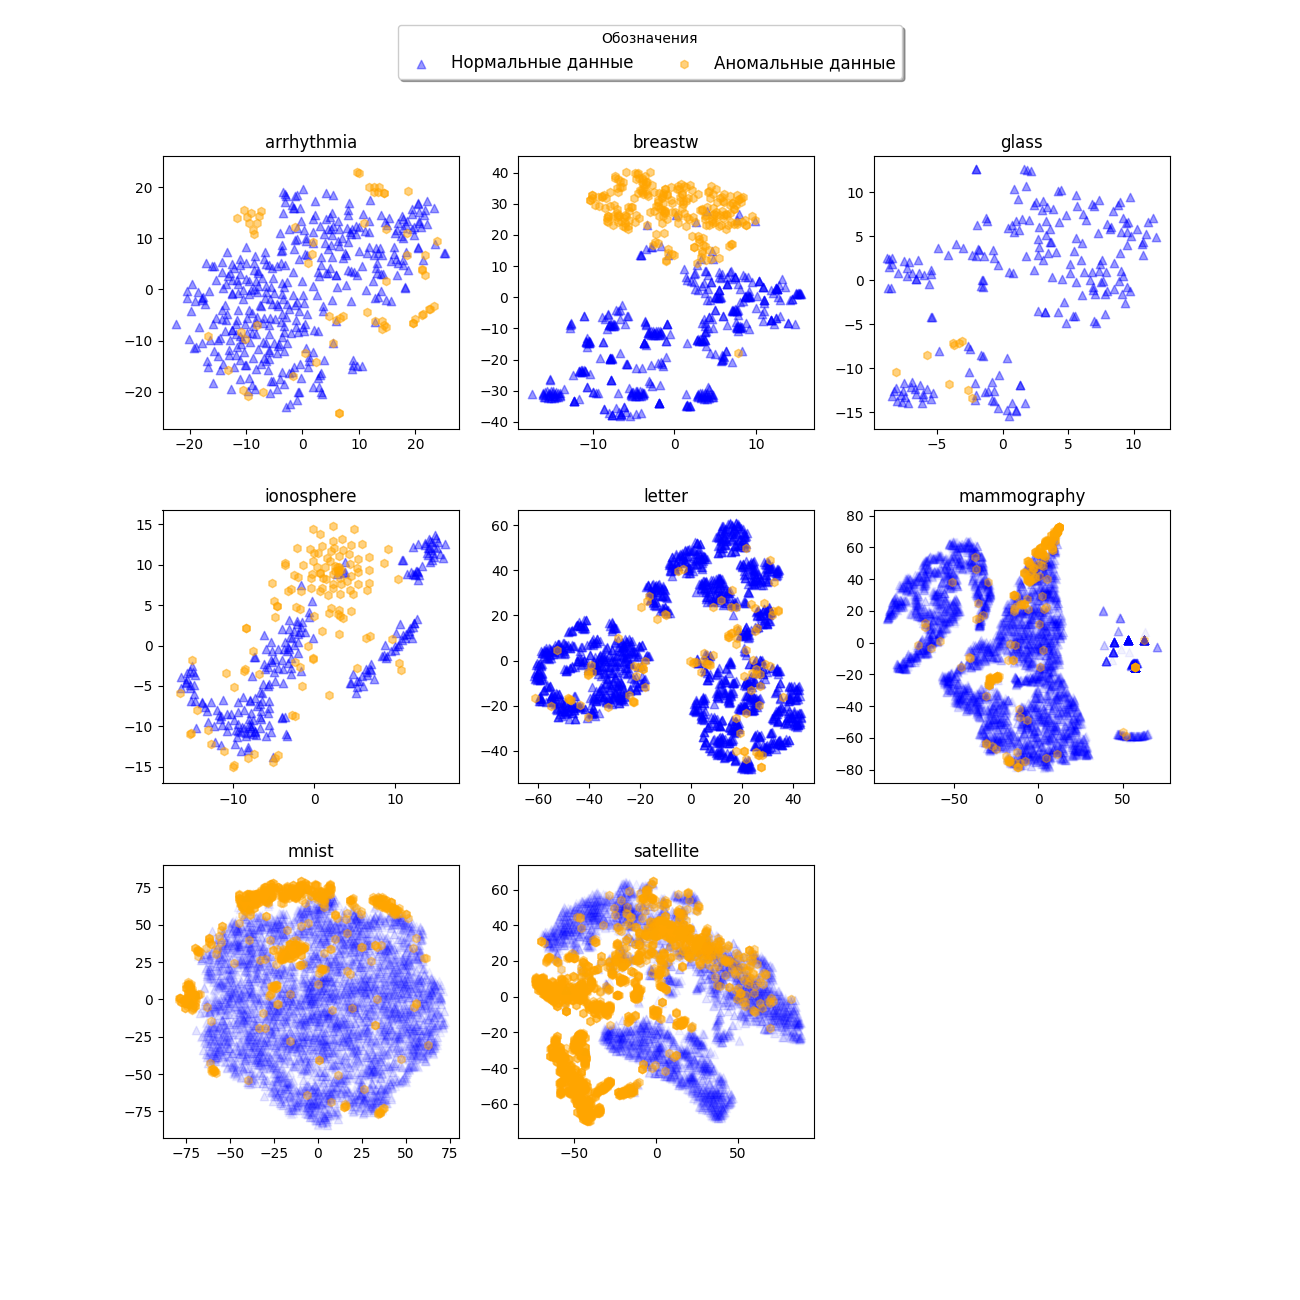
\includegraphics[width=\textwidth, height=\textheight, keepaspectratio] {2d_comparison}
  \caption{Рассматриваемые датасеты после применения алгоритма понижения размерности t-SNE.}
  \label{fig:2d_comparison}
\end{figure}

\begin{table} [htbp]
	\centering
	\caption{Значения ROC для рассматриваемых алгоритмов на данных.}\label{tab:rocs}%
	\begin{tabular}{lrrrrrr}
		\toprule
		     Датасет &   KNN &   PCA &  OCSVM &   LOF &  HBOS &  IFOREST \\
		\midrule   
   		arrhythmia &  0.7555 &  0.7794 &  0.7825 &  0.7672 &  0.7831 &   \textbf{0.7849} \\
     breastw &  \textbf{0.9908} &  0.9608 &  0.9649 &  0.4574 &  0.9764 &   0.9872 \\
       glass &  \textbf{0.8558} &  0.7308 &  0.8077 &  0.6538 &  0.7500 &   0.7212 \\
  ionosphere &  \textbf{0.9460} &  0.8115 &  0.8684 &  0.9023 &  0.6190 &   0.8632 \\
      letter &  \textbf{0.8660} &  0.5119 &  0.5985 &  0.8530 &  0.5532 &   0.5770 \\
 mammography &  0.8346 &  \textbf{0.9039} &  0.8911 &  0.6806 &  0.8506 &   0.8680 \\
       mnist &  0.8322 &  \textbf{0.8493} &  0.8487 &  0.6727 &  0.5607 &   0.7942 \\
   satellite &  0.6795 &  0.5601 &  0.6274 &  0.5567 &  \textbf{0.7464} &   0.7008 \\
		\bottomrule
		\hline
	\end{tabular}
\end{table}

\begin{figure}[ht]
  \centering
  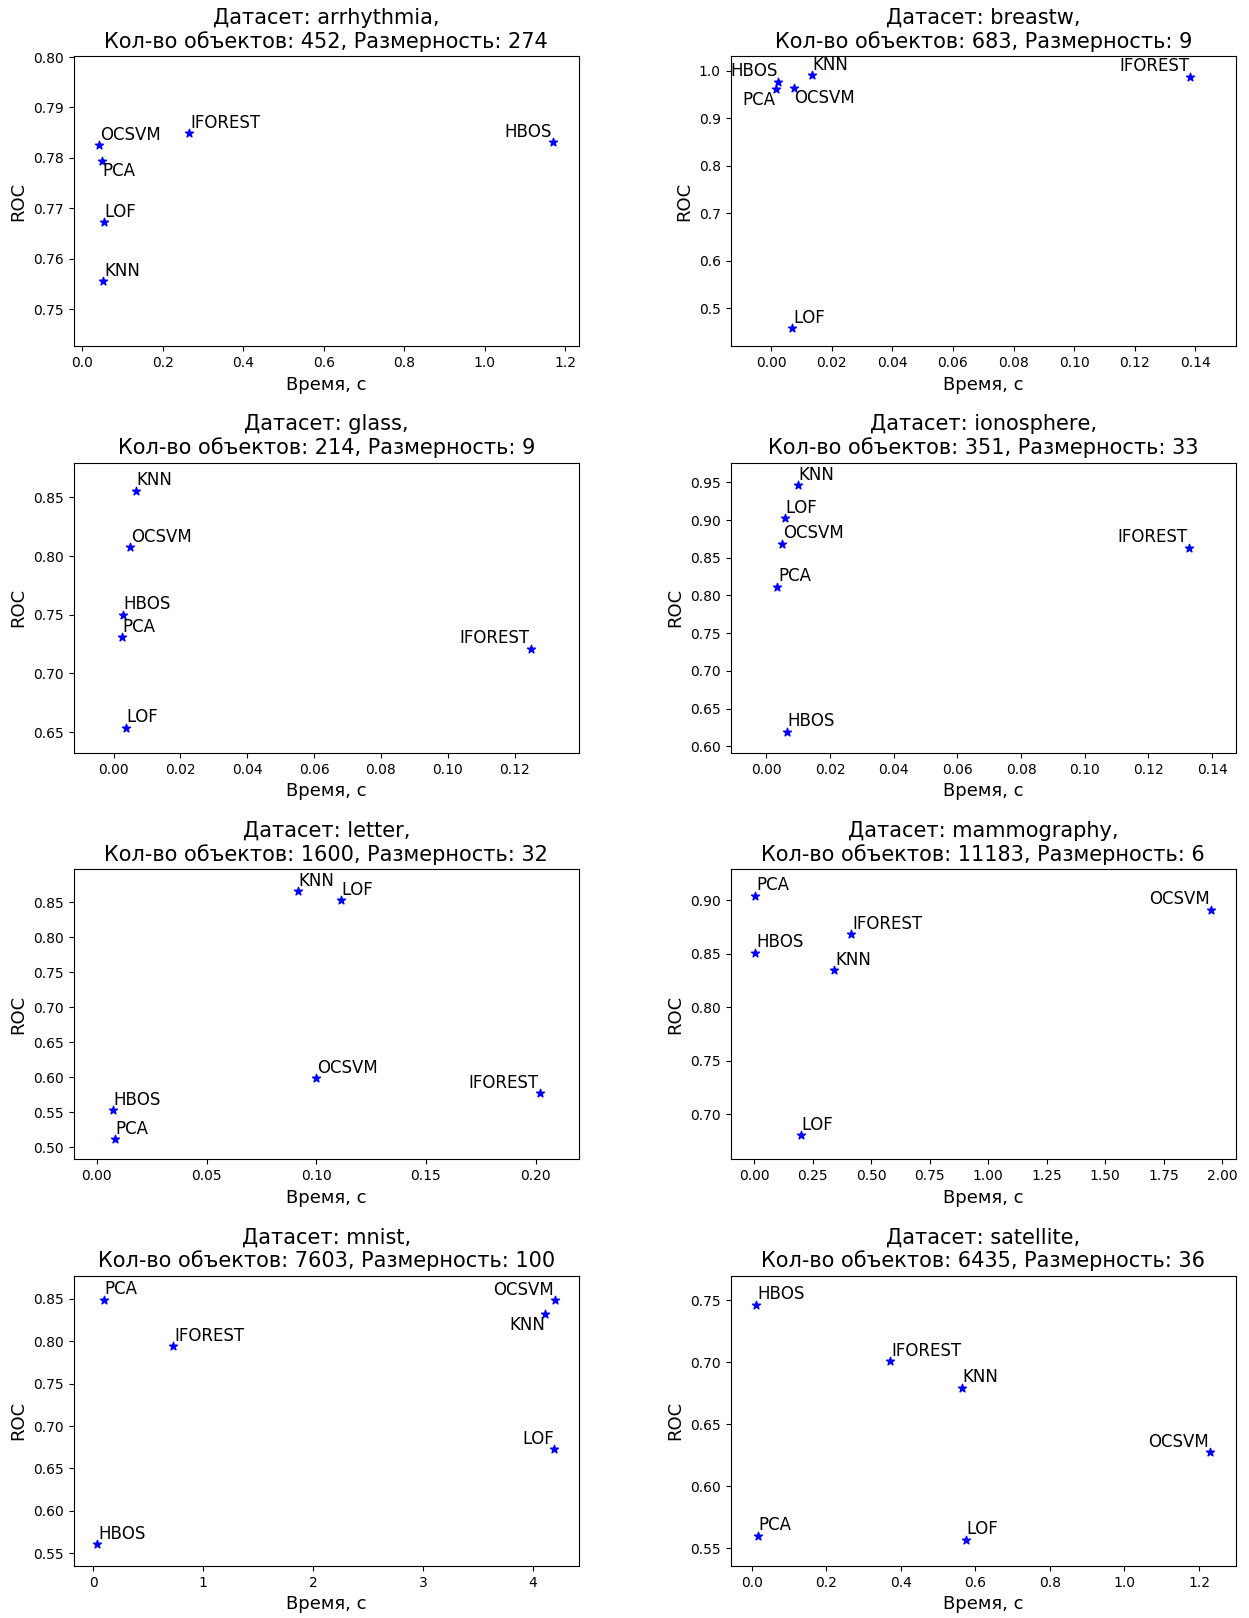
\includegraphics[width=\textwidth, height=\textheight, keepaspectratio] {roc_vs_time}
  \caption{Эффективность алгоритмов на разных датасетах.}
  \label{fig:roc_vs_time}
\end{figure}

При построении графиков, которые изображены на рисунке~\ref{fig:roc_vs_time}, использовалась библиотека adjustText\footnote{\url{https://github.com/Phlya/adjustText/}}.

\begin{figure}[ht]
  \centering
  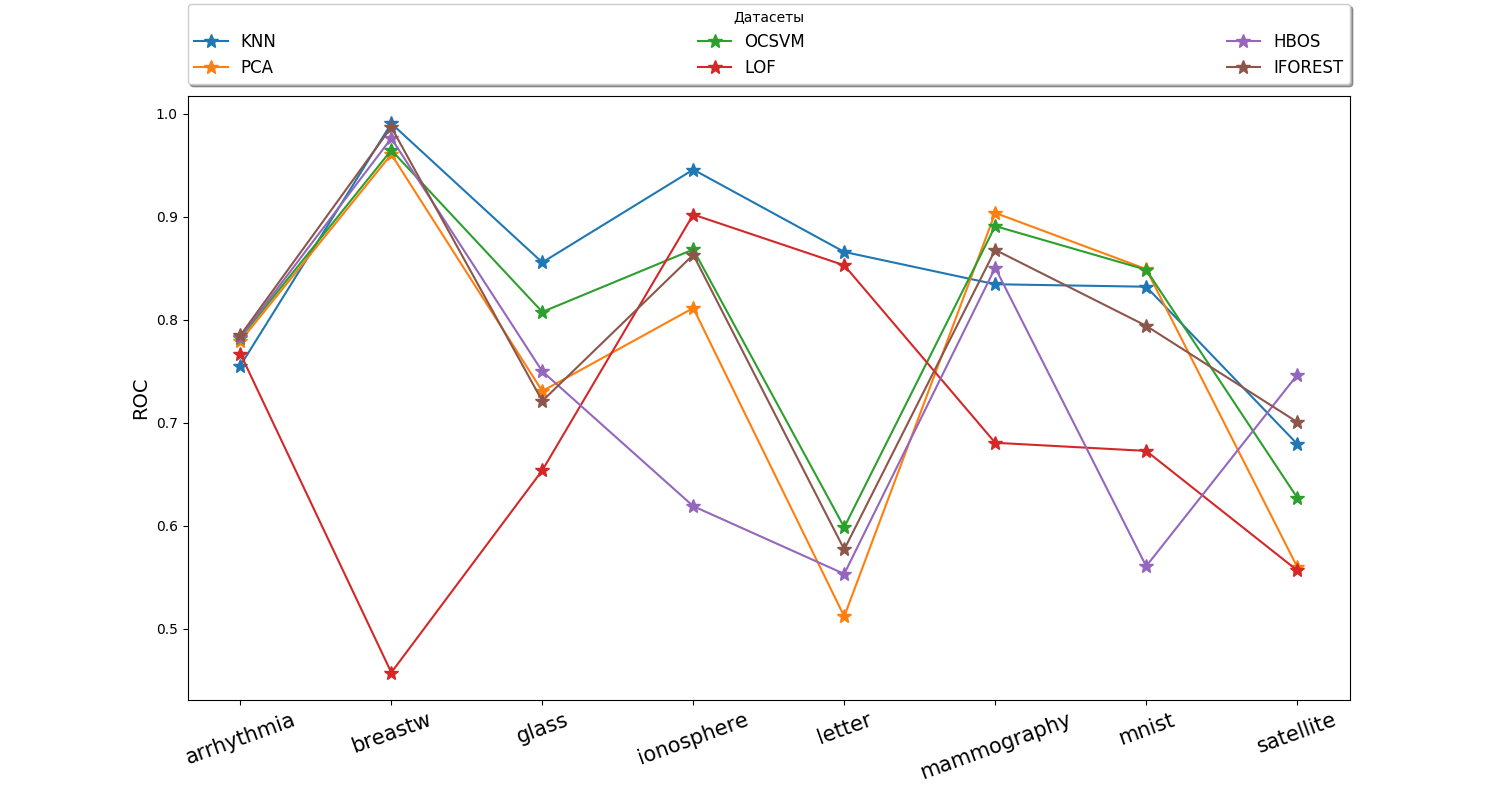
\includegraphics[width=\textwidth, height=\textheight, keepaspectratio] {roc_vs_dataset}
  \caption{Качество алгоритмов в зависимости от датасета.}
  \label{fig:roc_vs_dataset}
\end{figure}

Демонстрация наилучших результатов работы алгоритмов (рисунок~\ref{fig:d_breastw}).

\begin{figure}[ht]
  \centering
  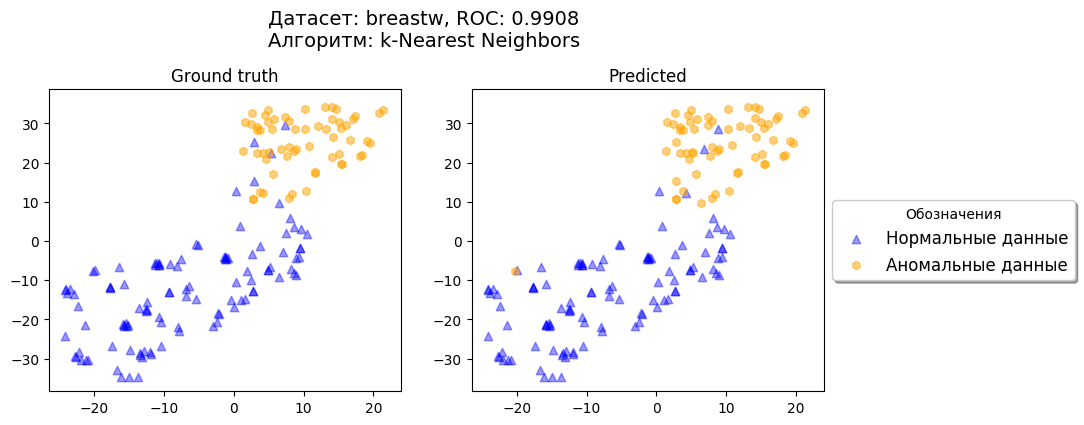
\includegraphics[width=\textwidth, height=\textheight, keepaspectratio] {d_breastw}
  \caption{Датасет Breast Cancer.}
  \label{fig:d_breastw}
\end{figure}

\clearpage

%\begin{figure}[ht]
%  \centering
%  
\includegraphics [scale=0.27] {latex}
%  \caption{TeX.}
%  \label{fig:latex}
%\end{figure}
